% 126-62(126쪽) — 자전거의 속도 v(t) km/h 의 그래프(위로 볼록한 이차함수). 스캔 화질이 낮아 TikZ 로 다시 그림.
% 원문에 있는 것만: 라벨 v(t) · t · O, t 눈금 2 와 4, v 눈금 40, 최고점으로 가는 가로·세로 안내 파선.
% 2 · 4 · 40 은 발문에 그대로 적혀 있는 값이라 그림에만 있는 정보가 아니다. 그 밖의 눈금은 넣지 않는다.
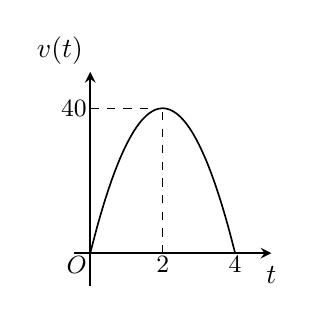
\begin{tikzpicture}[x=0.46cm, y=0.046cm, line width=0.5pt,
  tick/.style={font=\small, inner sep=1pt}]
  \draw[->, >=stealth, line width=0.7pt] (-0.45,0) -- (5.0,0) node[below=1pt] {$t$};
  \draw[->, >=stealth, line width=0.7pt] (0,-9) -- (0,50) node[above left=-1pt] {$v(t)$};
  \node[tick, below left] at (0,0) {$\pt{O}$};
  % 최고점 안내 파선(원문)
  \draw[dashed, line width=0.35pt] (0,40) -- (2,40);
  \draw[dashed, line width=0.35pt] (2,0) -- (2,40);
  % 그래프 — 위로 볼록, t=0 과 t=4 에서 t축과 만나고 t=2 에서 최고
  \draw[line width=0.6pt, smooth] plot coordinates
    {(0,0) (0.2,7.6) (0.4,14.4) (0.6,20.4) (0.8,25.6) (1.0,30.0) (1.2,33.6) (1.4,36.4)
     (1.6,38.4) (1.8,39.6) (2.0,40.0) (2.2,39.6) (2.4,38.4) (2.6,36.4) (2.8,33.6)
     (3.0,30.0) (3.2,25.6) (3.4,20.4) (3.6,14.4) (3.8,7.6) (4.0,0)};
  \node[tick, below] at (2,0) {$2$};
  \node[tick, below] at (4,0) {$4$};
  \node[tick, left] at (0,40) {$40$};
\end{tikzpicture}
